%-----------------------------------------------------------------------------------------------------------------------------------------------%
%	The MIT License (MIT)
%
%	Copyright (c) 2015 Jan Küster
%
%	Permission is hereby granted, free of charge, to any person obtaining a copy
%	of this software and associated documentation files (the "Software"), to deal
%	in the Software without restriction, including without limitation the rights
%	to use, copy, modify, merge, publish, distribute, sublicense, and/or sell
%	copies of the Software, and to permit persons to whom the Software is
%	furnished to do so, subject to the following conditions:
%	
%	THE SOFTWARE IS PROVIDED "AS IS", WITHOUT WARRANTY OF ANY KIND, EXPRESS OR
%	IMPLIED, INCLUDING BUT NOT LIMITED TO THE WARRANTIES OF MERCHANTABILITY,
%	FITNESS FOR A PARTICULAR PURPOSE AND NONINFRINGEMENT. IN NO EVENT SHALL THE
%	AUTHORS OR COPYRIGHT HOLDERS BE LIABLE FOR ANY CLAIM, DAMAGES OR OTHER
%	LIABILITY, WHETHER IN AN ACTION OF CONTRACT, TORT OR OTHERWISE, ARISING FROM,
%	OUT OF OR IN CONNECTION WITH THE SOFTWARE OR THE USE OR OTHER DEALINGS IN
%	THE SOFTWARE.
%	
%
%-----------------------------------------------------------------------------------------------------------------------------------------------%

% we use report class for thesis design
% 11pt font is way bettern to read than 12pt
% we want to make a title page
% two side allows us to make the page layout align by even and odd
% openright tells the compiler that the first page is a right page
\documentclass[pdftex,11pt,titlepage,twoside,openright]{article} 


%--------\usepackage{listings}--------------------------------------------------------------------------------
%	ENCODING
%----------------------------------------------------------------------------------------

% for suporting multi platform
\usepackage[utf8x]{inputenc}

% natbib is what you want for bibliography
\usepackage[square,authoryear]{natbib}


%-----------------------------------------------------------------------------------------------------------------------------------------------%
% INCLUDE CONFIGURATION
%-----------------------------------------------------------------------------------------------------------------------------------------------%



%----------------------------------------------------------------------------------------
%	FONT
%----------------------------------------------------------------------------------------

% some tex-live fonts - choose your own

%\usepackage[defaultsans]{droidsans}
%\usepackage[default]{comfortaa}
%\usepackage{cmbright}
\usepackage[default]{raleway}
%\usepackage{fetamont}
%\usepackage[default]{gillius}
%\usepackage[light,math]{iwona}
%\usepackage[thin]{roboto} 

% set font default
\renewcommand*\familydefault{\sfdefault} 	
\usepackage[T1]{fontenc}

% more font size definitions
\usepackage{moresize} 

%----------------------------------------------------------------------------------------
%	COLORS
%----------------------------------------------------------------------------------------

\usepackage{color}

\definecolor{arsenic}{rgb}{0.23, 0.27, 0.29}
\definecolor{coolblack}{rgb}{0.0, 0.18, 0.39}

%----------------------------------------------------------------------------------------
%	CODE SYNTAX HIGHLIGHT
%----------------------------------------------------------------------------------------

% thanks to: http://tex.stackexchange.com/questions/89574/language-option-supported-in-listings

\usepackage{listings}


\definecolor{lightgray}{rgb}{.9,.9,.9}
\definecolor{darkgray}{rgb}{.4,.4,.4}
\definecolor{purple}{rgb}{0.65, 0.12, 0.82}

\lstdefinelanguage{JavaScript}{
  keywords={typeof,instanceof, new, true, false, catch, function, return, null, catch, switch, var, if, in, while, do, else, case, break, of, const, let},
  keywordstyle=\color{orange}\bfseries,
  ndkeywords={class, export, boolean, throw, implements, import, this},
  ndkeywordstyle=\color{orange}\bfseries,
  identifierstyle=\color{black},
  sensitive=false,
  comment=[l]{//},
  morecomment=[s]{/*}{*/},
  commentstyle=\color{gray}\ttfamily,
  stringstyle=\color{coolblack}\ttfamily,
  morestring=[b]',
  morestring=[b]",
 xleftmargin=0.7cm, xrightmargin=0.5cm,
 rulesepcolor=\color{black},
 showspaces=false,showtabs=false,tabsize=2,
 numberstyle=\tiny,numbers=left,
}

\lstset{
   language=JavaScript,
   backgroundcolor=\color{lightgray},
   extendedchars=true,
   basicstyle=\footnotesize\ttfamily,
   showstringspaces=false,
   showspaces=false,
   numbers=left,
   numberstyle=\footnotesize,
   numbersep=9pt,
   tabsize=2,
   breaklines=true,
   showtabs=false,
   captionpos=b
}





% RECREATE FRAME TO NOTHING SO WE CAN JUST INCLUDE IT AS IT IS
\renewenvironment{frame}{}{}

% replacement for \frametitle
\newcommand{\frametitle}[1]{\subsection{#1}}

% replacement for \pause
\newcommand{\pause}{\newline}


\newcommand{\subtitle}[1]{#1}

\newcommand{\institute}[1]{#1}

\newcommand{\inst}[1]{}

\renewcommand{\and}{and}

\newcommand{\subject}[1]{{#1}}

\newcommand{\only}[1]{\item #1}

\renewcommand{\itemize}[1]{
	\renewcommand{\item}[1]{#1}
}{}


\usepackage{graphicx}

\usepackage{xcolor}

\newenvironment{columns}[3]{}{}

\newenvironment{column}[4]{}{}

\newenvironment{block}[2]{
	\textbf{\uppercase{#1}}\\
	#2\hspace{-2pt}}{}

\newenvironment{alertblock}[2]{
	\textbf{\uppercase{#1}}\\
	#2\hspace{-3pt}}{}

\newenvironment{exampleblock}[2]{
	\textbf{\uppercase{#1}}\\
	#2\hspace{-3pt}}{}


\usepackage{lastpage}

\newcommand{\insertframenumber}{\thepage}
\newcommand{\inserttotalframenumber}{\thepage}

\input{./config/title-common.tex}

\begin{document}

\input{./config/title-handouts.tex}
\maketitle
\newpage

\tableofcontents
\newpage


\section{Standard Slides}

\subsection{Text Only}

\begin{frame}
	\frametitle{Default Text Slide}
	%Content goes here
	Vero minima pariatur ea itaque natus in. In quidem non error fugiat tempore aliquid magni. Animi aliquam voluptatum eum. Delectus voluptate illum quidem et autem.
\end{frame}

\subsection{Lists}

\begin{frame}
	\frametitle{Itemize and Listing}
	%Content goes here
	Vero minima pariatur ea itaque natus in. In quidem non error fugiat tempore aliquid magni. Animi aliquam voluptatum eum.
	\pause
	 Delectus voluptate illum quidem et autem.

	\begin{itemize}[<+->]
		\item This one is always shown
		\item The first time (i.e. as soon as the slide loads)
		\item The second time
		\item Also the first time
		\only {This one is shown at the first time, but it will hide soon (on the next event after the slide loads).}
	\end{itemize}
\end{frame}

\subsection{Graphics}

\frame[plain]{
	\frametitle{Include an Image}
	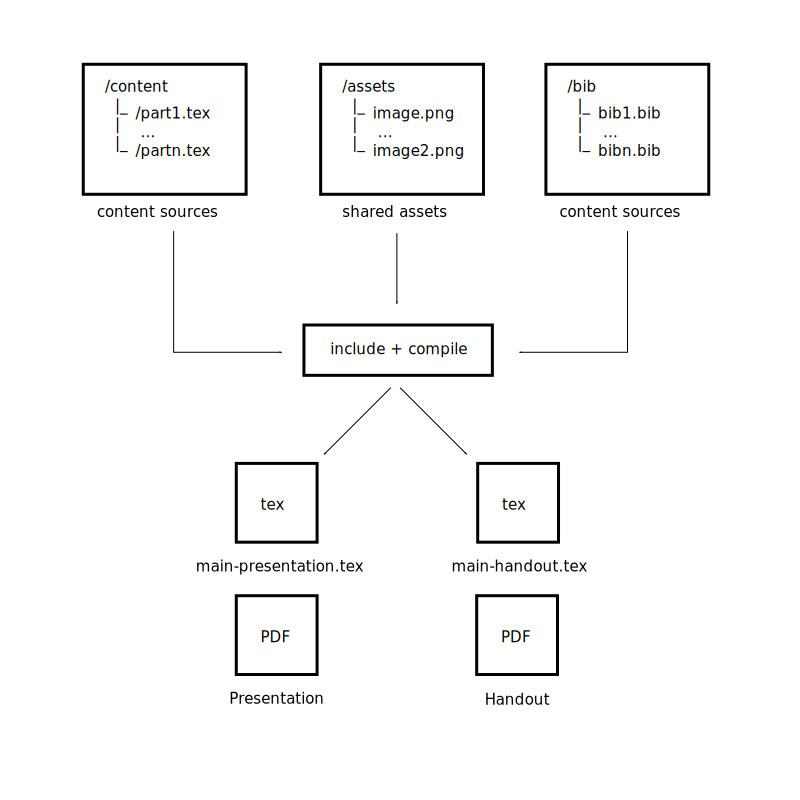
\includegraphics[width=0.5\linewidth]{./assets/overview.png}
}

\section{Include Source Code}

\begin{frame}[fragile]
\frametitle{Some Simple C Code}

\begin{lstlisting}[caption=Some JavaScript code]
var x = 3;
var y = 5;

this.bla;
var obj = new Object();

/**
 * Adds to variables and returns the result.
 **/
obj.add = function(a, b) {
	return a + b;
};

var z = obj.add(x, y);

console.log("bla");

\end{lstlisting}
\end{frame}

\section{Columns on Slides}

\begin{frame}
	\frametitle{Example of columns 2}
	\begin{columns}[T] % contents are top vertically aligned
	\begin{column}[T]{5cm} % each column can also be its own environment
	Contents of first column \\ split into two lines \\
	Pagenumbers: \insertframenumber/\inserttotalframenumber
	\end{column}
	\begin{column}[T]{5cm} % alternative top-align that's better for graphics
          		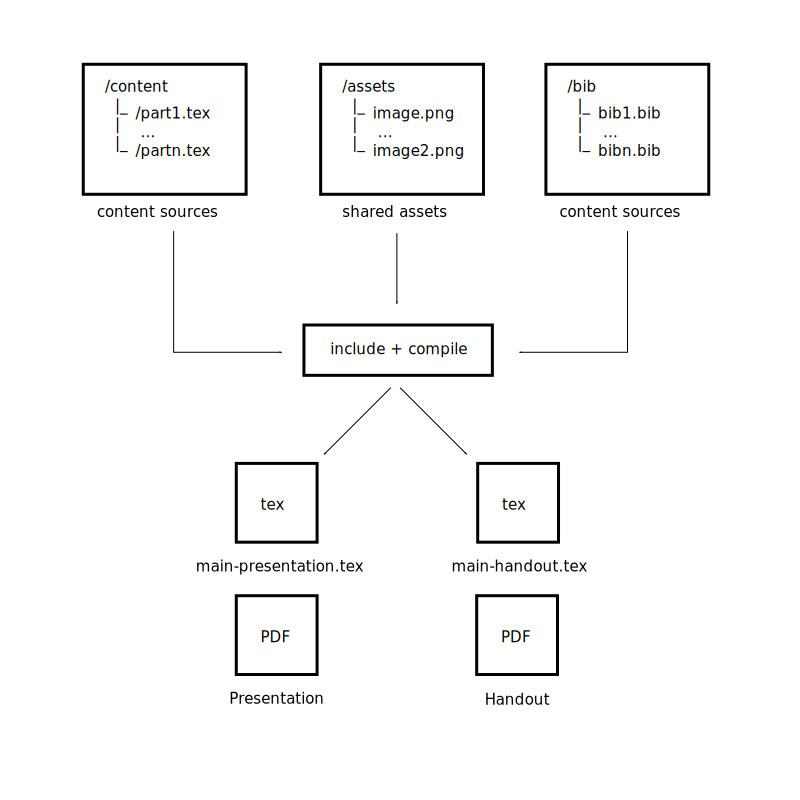
\includegraphics[height=3cm]{./assets/overview.png}
	\end{column}
	\end{columns}
\end{frame}


\section{Blocks on Slides}


\begin{frame}

   \begin{block}{This is a Block}
      This is important information
   \end{block}

   \begin{alertblock}{This is an Alert block}
   This is an important alert
   \end{alertblock}

   \begin{exampleblock}{This is an Example block}
   This is an example 
   \end{exampleblock}

\end{frame}


\end{document}